\chapter{Related Work}

\section{CTR Prediction}

Current click-through rate (CTR) prediction methods can be categorized into two main types: \textit{feature engineering} and \textit{model engineering}.

\subsection{Feature Engineering}

Feature engineering focuses on mining and selecting informative features relevant to CTR prediction. These features include graph features, visual features, textual features, and multimodal features. For example, some methods collect textual descriptions of features, encode the text using pretrained language models (PLMs) to obtain semantic embeddings, and employ alignment loss to align collaborative signals with these embeddings.

Several studies have also focused on filtering out noisy or irrelevant features using automated selection or attention-based methods.

\subsection{Model Engineering}

Model engineering aims to design more effective models to extract information from the input features. This includes developing diverse types of feature interactions, such as Factorization Machines (FM), DeepFM, EulerNet, and KAN.

In addition, many works model user interests—especially long- and short-term interests—based on behavior sequences. These techniques aim to dynamically capture evolving user preferences and improve recommendation quality.

This study falls under the category of feature engineering. Specifically, we mine multi-faceted knowledge from entangled textual information and integrate this knowledge into CTR prediction.

\section{Disentangled Representation Learning}

Disentangled representation learning (DRL) seeks to extract informative and independent factors of variation in data. It has gained significant attention due to its superior explainability.

\subsection{VAE-based Disentanglement}

VAE-based DRL methods can be divided into:
\begin{itemize}
    \item \textbf{Unsupervised approaches}, which re-weight or decompose the evidence lower bound (ELBO) of the VAE to encourage factor separation.
    \item \textbf{Supervised approaches}, which introduce weak supervision signals such as grouping or causal relationships to enforce disentanglement.
\end{itemize}

\subsection{DRL in Recommendation}

DRL for recommendation systems aims to enhance representation learning by separating latent aspects such as:
\begin{itemize}
    \item User interests (e.g., short-term vs. long-term).
    \item Multi-source inputs (e.g., user-item interaction vs. side information).
\end{itemize}

Compared to existing studies, our method focuses on disentangling semantic embeddings from textual side information and using the learned factors to guide CTR prediction.

\section{Topic Model}

Traditional topic models aim to discover latent semantic structures in document collections using probabilistic graphical models (e.g., LDA, dynamic topic models). These models typically infer topic-word and document-topic distributions using methods such as Gibbs sampling or variational inference.

With the success of VAE, neural topic models emerged, which combine the reparameterization trick with BoW-based document representation.

More recently, topic modeling has been extended to PLM-based semantic embeddings. Instead of representing documents as word-count vectors, these methods derive topic distributions from continuous text embeddings, allowing more nuanced topic extraction.

In our work, we propose a disentangled topic model that leverages both BoW structure and semantic embeddings to guide CTR learning.

\section{Comprehensive Related Work Analysis}

\subsection{Evolution of CTR Prediction Models}
\textbf{Early Approaches (2010-2015):} Traditional machine learning methods like logistic regression and gradient boosting dominated.

\textbf{Deep Learning Era (2016-2020):} Introduction of neural networks brought significant improvements~\cite{guo2017deepfm}.

\textbf{Attention Mechanisms (2018-2021):} Models like DIN~\cite{zhou2018deep} and DIEN~\cite{zhou2019deep} introduced attention for user interest modeling.

\textbf{Pre-trained Models (2021-Present):} Integration of large language models represents the current frontier~\cite{wang2023bert4ctr}.

\subsection{Topic Modeling Landscape}
\textbf{Classical Methods:} LDA~\cite{blei2003latent}, CTM~\cite{blei2006dynamic}, and HDP provided foundational approaches.

\textbf{Neural Topic Models:} VAE-based approaches like NVDM and ETM~\cite{dieng2020topic} enabled end-to-end learning.

\textbf{Pre-trained Topic Models:} Recent work like BERTopic~\cite{grootendorst2022bertopic} leverages transformer embeddings.

\subsection{Disentanglement in Recommendation}
Detailed comparison of disentanglement approaches:
\begin{itemize}
    \item \textbf{Factor-based Methods}~\cite{ma2019learning}: Separate collaborative signals into independent factors
    \item \textbf{Multi-task Learning}: Use auxiliary tasks to encourage disentanglement
    \item \textbf{Causal Approaches}~\cite{yang2021causalvae}: Model causal relationships between latent factors
\end{itemize}

\section{Qualitative Study}

\subsection{Visualization of Learned Embeddings}

To evaluate the quality of the learned semantic representations, we visualize different models' embeddings using t-SNE. We compare:
\begin{itemize}
    \item Disentangled topic embeddings from \textbf{DSTopic}.
    \item Disentangled semantic embeddings from \textbf{TopicDRL}.
    \item Naive concat embeddings.
    \item Other methods such as \textbf{TIGER}, \textbf{VQRec}, and \textbf{MoC}.
\end{itemize}

\begin{figure}[htbp]
    \centering
    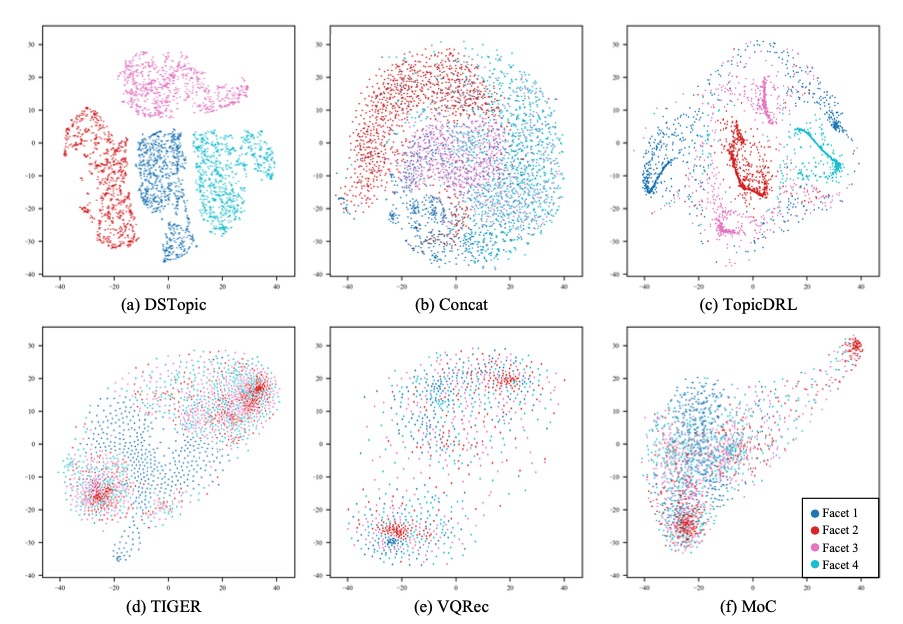
\includegraphics[width=\textwidth]{Figures/Chapter5/fig3.png}
    \caption{Visualization of learned semantic embeddings using DCNv2 on the Garden dataset.}
    \label{fig:tsne}
\end{figure}

We observe that DSTopic and TopicDRL both learn well-separated and interpretable semantic spaces, while other baselines suffer from entanglement or overlap in latent space.

\subsection{Effect of Number of Views}

We vary the number of semantic views $H \in \{1, 2, 4, 6, 8\}$ and compare MSD-CTR against the naive concat method on the Garden dataset. The metrics used are AUC and LogLoss.

\begin{figure}[htbp]
    \centering
    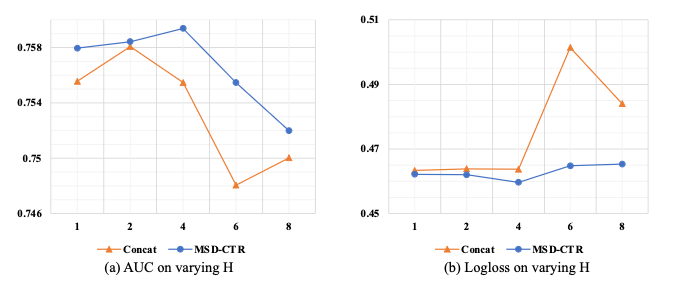
\includegraphics[width=\textwidth]{Figures/Chapter5/fig4.png}
    \caption{Performance comparison on different number of semantic views $H$ for MSD-CTR and Concat.}
    \label{fig:view-ablation}
\end{figure}

Results show that:
\begin{itemize}
    \item MSD-CTR benefits from disentangling semantic knowledge into multiple views.
    \item When $H$ becomes too large, performance drops due to over-fragmentation.
    \item Concat degrades faster due to view overlap and multicollinearity.
\end{itemize}
